%\documentclass[draft,aspectratio=169]{beamer}
\documentclass[aspectratio=169]{beamer}
% http://deic.uab.es/~iblanes/beamer_gallery/index_by_theme.html
%
\mode<presentation>
{
    \usetheme{Montpellier}      % or try Darmstadt, Madrid, Warsaw, ...
    \usecolortheme{beaver} % or try albatross, beaver, crane, ...
    \usefonttheme{default}  % or try serif, structurebold, ...
    \setbeamertemplate{navigation symbols}{}
    \setbeamertemplate{caption}[numbered]
} 

\usepackage[english]{babel}
\usepackage[utf8]{inputenc}
\usepackage[T1]{fontenc}
\usepackage{amsmath}
\usepackage[framemethod=TikZ]{mdframed}

\input{/home/istvan/insar/latex_aux.tex}

\newcommand{\imp}[1]{ {\Large \color{red} \textbf{#1}} }

\newcommand{\fig}[1]{
    \begin{mdframed}[linecolor=red!50!black, linewidth=2pt, roundcorner=2.25pt,
                     innerrightmargin=0pt, innerleftmargin=0pt,
                     innertopmargin=0pt, innerbottommargin=0pt,
                     backgroundcolor=white, frametitle={}, align=center]
        \includegraphics[width=1.0\textwidth]{#1}
    \end{mdframed}
}

\graphicspath{{/home/istvan/insar/images/}}

\title[InSAR]{An attempt to apply space-borne monitoring of recent tectonics in the Southern Carpathians}
\author{István Bozsó, László Bányai, Eszter Szűcs, Viktor Wesztergom}
\institute{MTA CSFK Geodetic and Geophysical Institute}
\date{2018.09.11.}

\begin{document}

\begin{frame}
    \titlepage
    \begin{center}
        \begin{minipage}[c]{0.25\textwidth}
            
\includegraphics[width=0.75\textwidth]{ggi_logo.png}
        \end{minipage}
        \hspace{25pt}
        \begin{minipage}[c]{0.25\textwidth}
            
\includegraphics[width=0.75\textwidth]{esa_logo.eps}
        \end{minipage}
    \end{center}
\end{frame}

\begin{frame}{Outline}
    \tableofcontents
\end{frame}

\section{Introduction}

\subsection{Motivation}

\begin{frame}{Motivation}
\begin{itemize}
    \pause
    \item Validation of geodynamic models? $\rightarrow$ large databases needed
    \pause
    \item GPS networks: too sparse and not cost effective
    \pause
    \item tilt meters: expensive (instrument + borehole), time series from a single point only
    \pause
    \item Solution? \pause $\rightarrow$ space geodesy \pause $\rightarrow$ InSAR
\end{itemize}
\end{frame}

\subsection{Basics of interferometry}

\begin{frame}{Range change detection with interferometry}

    \begin{minipage}[c]{0.45\textwidth}
        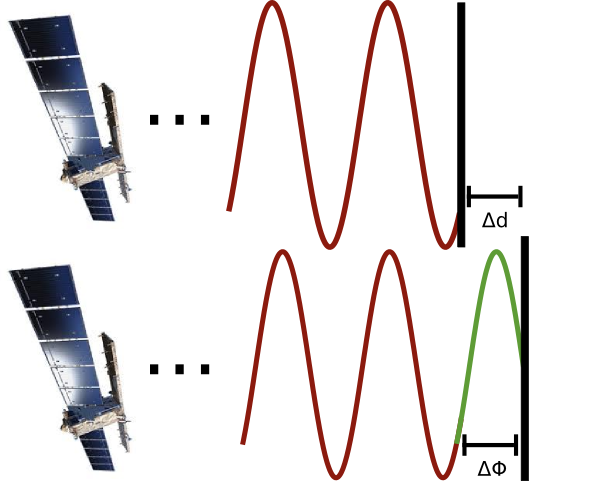
\includegraphics[width=\textwidth]{interfero.png}
    \end{minipage}
    \hspace{15pt}
    \begin{minipage}[c]{0.45\textwidth}
        \pause
        \[
            \highlight{\Delta \mathbf{d}}{red!60} \cdot \highlight{\mathbf{n}}{orange} = - \frac{\lambda}{4 \pi} \highlight{\Delta \Phi}{green!60}
        \]
        $\mathbf{n}$: normal vector of wave propagation
        \vspace{15pt}

        \pause
        \imp{Only changes in range are detected, not absolute range!}
        \vspace{15pt}

        \pause
        \imp{Movements perpendicular to the direction of wave propagation do not produce phase change!}
    \end{minipage}
\end{frame}

\begin{frame}{Phase unwrapping}
    \pause
    \begin{minipage}[c]{0.575\textwidth}
        \centering
        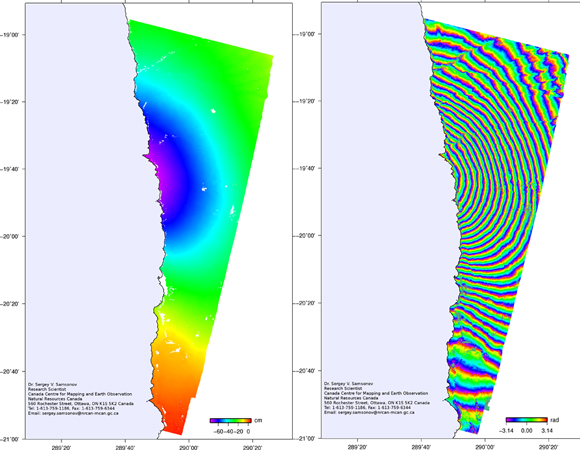
\includegraphics[width=\textwidth]{wrapped_and_unwrapped_ifg.jpg}
        
        {\tiny Figure source: https://www.unavco.org/highlights/2014/iquique.html}
    \end{minipage}
    \hspace{5pt}
    \begin{minipage}[c]{0.35\textwidth}
        \pause
        Wrapped phase (left) and Unwrapped phase (right).
        \vspace{10pt}
        \pause
        \imp{If the change in range is larger than half wavelength between two
             measurements the reconstruction of the unwrapped phase is uncertain at best!}
    \end{minipage}
\end{frame}

\subsection{Summary}

\begin{frame}{Summary}
    \pause
    \begin{block}{Rule 1}
        Relative technique: only changes in range are detected, not absolute range.
    \end{block}
    \vspace{10pt}
    \pause
    \begin{block}{Rule 2}
        Movements perpendicular to the direction of wave propagation do not produce phase change.
    \end{block}
    \vspace{10pt}
    \pause
    \begin{block}{Rule 3}
        Phase unwrapping is uncertain when $\Delta \mathrm{d} > \frac{\lambda}{2}$ between two measurements.
    \end{block}
\end{frame}

\section{InSAR - geoscientific applications}

\subsection{Time series analysis}

\begin{frame}{Absence of scatterers}
    \begin{minipage}[t]{0.62\textwidth}
        \fig{antropo_overw.png}
    \end{minipage}
    \hspace{15pt}
    \begin{minipage}[t]{0.32\textwidth}
        \fig{antropo_los_mod.png}
        
        \vspace{10pt}
        {\LARGE Average displacement velocities in Berlin, Germany}
    \end{minipage}
\end{frame}

\subsection{Observing slow geodynamic processes with reflectors}

\begin{frame}{Twin reflectors for ascending and descending measurments}
    \begin{minipage}[c]{0.45\textwidth}
        \centering
        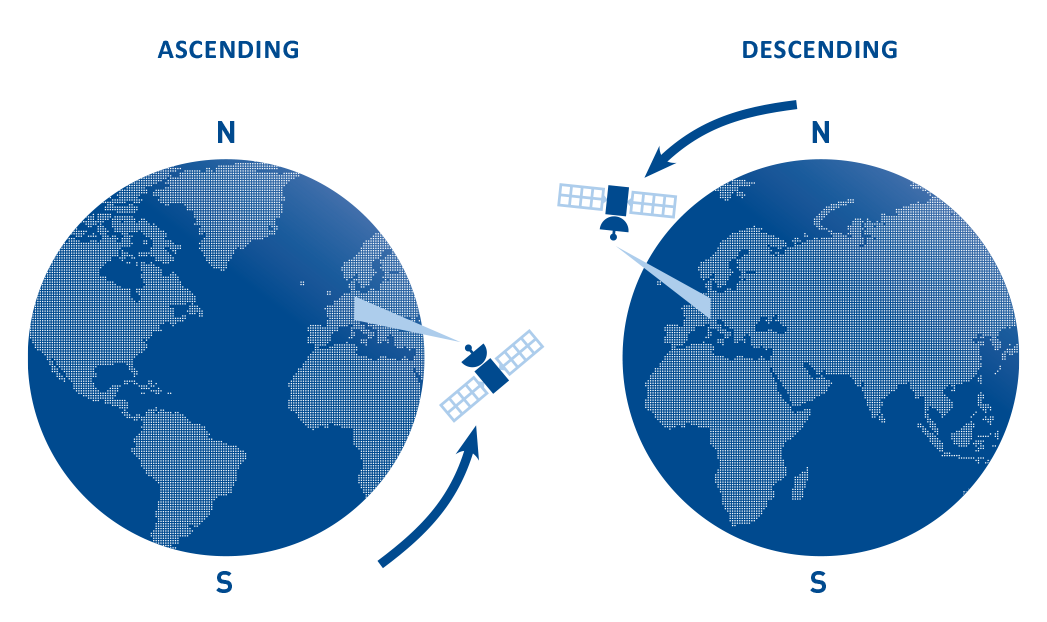
\includegraphics[width=\textwidth]{ascending_descending_orbits.png}
        
        Ascending and descending satellite orbits.
    \end{minipage}
    \hspace{15pt}
    \pause
    \begin{minipage}[c]{0.45\textwidth}
        \centering
        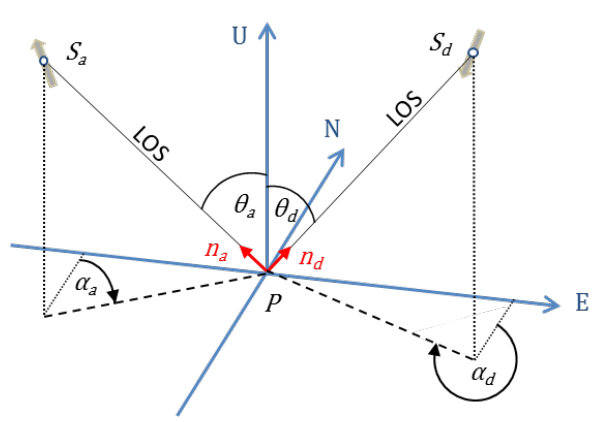
\includegraphics[width=\textwidth]{daisy_schematic.png}
        
        Geometry of satellite orbits with repsect to a surface scatterer.
    \end{minipage}    
\end{frame}

\begin{frame}{Twin reflectors for ascending and descending measurments}
    \pause
    \textbf{ESA PECS project $\rightarrow$ design, installment and testing of reflector benchmarks.}
    \vspace{10pt}
    
    \begin{minipage}[c]{0.35\textwidth}
        \pause
        \underline{Aspects of reflector design:}
        \begin{itemize}
            \pause
            \item analogue, analytical and numerical calculations,
            \item Sentinel-1 observing wavelength and orbit parameters,
            \item mechanical compactness and robustness
        \end{itemize}
        \pause
        \begin{center}
            \resizebox{0.15\textwidth}{10pt}{$\Downarrow$}
            
            optimal reflector size and parameters.
        \end{center}
    \pause
    \end{minipage}
    \hspace{10pt}
    \begin{minipage}[c]{0.55\textwidth}
        \fig{dszekcso_refl_2.jpg}
        Installed reflector at Dunaszekcső with GNSS receiver.
    \end{minipage}    
\end{frame}

\begin{frame}{Installed reflectors in Hungary}
    \begin{minipage}[c]{0.775\textwidth}
        \fig{hungary_networks.png}
    \end{minipage}
    \hspace{10pt}
    \begin{minipage}[c]{0.1575\textwidth}
        {\LARGE Reflector networks in Hungary}
    \end{minipage}
\end{frame}


\begin{frame}{Installed reflectors in Hungary}
    \begin{minipage}[c]{0.365\textwidth}
        \centering
        \fig{dszekcso_network.png}

        Dunaszekcső network
    \end{minipage}
    \hspace{10pt}
    \begin{minipage}[c]{0.58\textwidth}
        \centering
        \fig{kulcs_network.png}

        Kulcs network
    \end{minipage}
\end{frame}

\begin{frame}{First results of benchmarks - Dunaszekcső}
    \begin{minipage}[t]{0.485\textwidth}
        \centering
        \includegraphics[width=\textwidth]{dszekcso_asc_dsc.eps}
        \vspace{10pt}
        LOS deformation in the ascending (ASC) and descending (DSC) direction.
    \end{minipage}
    \hspace{5pt}
    \begin{minipage}[t]{0.485\textwidth}
        \centering
        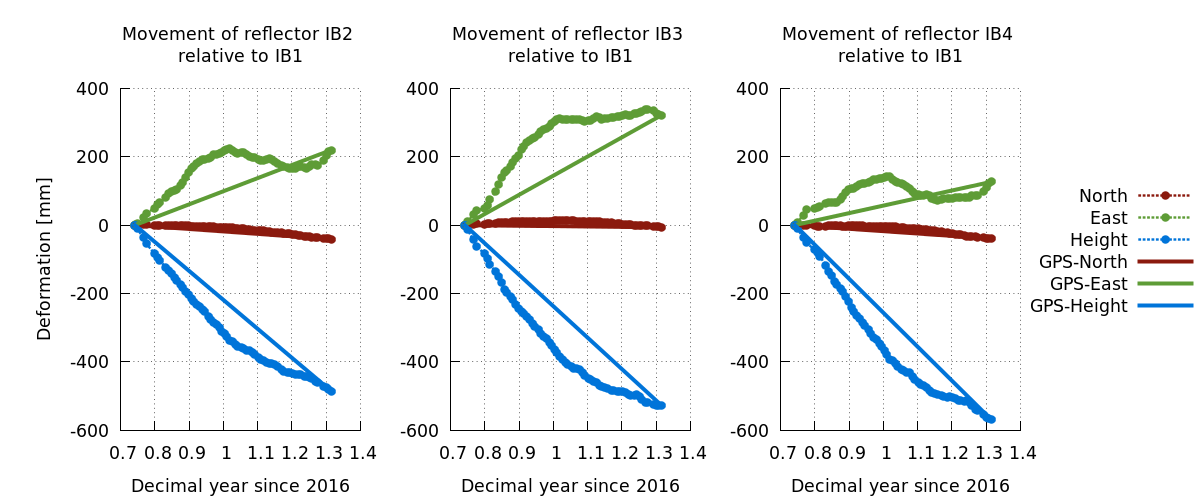
\includegraphics[width=\textwidth]{dszekcso_kalman.eps}
        \vspace{10pt}
        Result of Kalman-filtering = Sentinel-1 data + GPS measurements.
    \end{minipage}
\end{frame}

\begin{frame}{First results of benchmarks - Kulcs}
    \begin{minipage}[t]{0.485\textwidth}
        \centering
        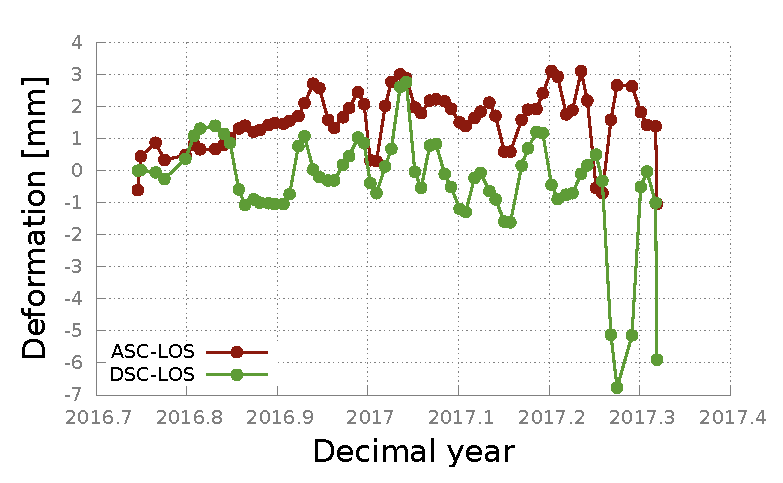
\includegraphics[width=\textwidth]{kulcs_asc_dsc.eps}
        \vspace{10pt}
        LOS deformation in the ascending (ASC) and descending (DSC) direction.
    \end{minipage}
    \hspace{5pt}
    \begin{minipage}[t]{0.485\textwidth}
        \centering
        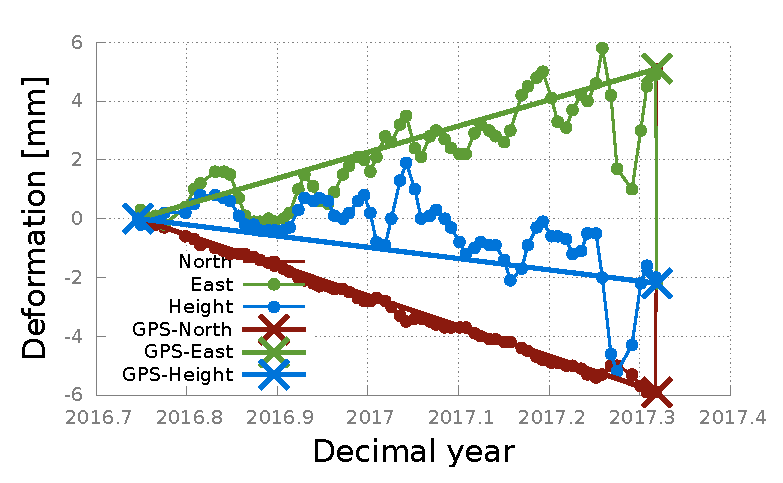
\includegraphics[width=\textwidth]{kulcs_kalman.eps}
        \vspace{10pt}
        Result of Kalman-filtering = Sentinel-1 data + GPS measurements.
    \end{minipage}
\end{frame}

\section{TopoTransylvania and future reflector networks}

\begin{frame}{TopoTransylvania project}
    \begin{minipage}[c]{0.54\textwidth}
        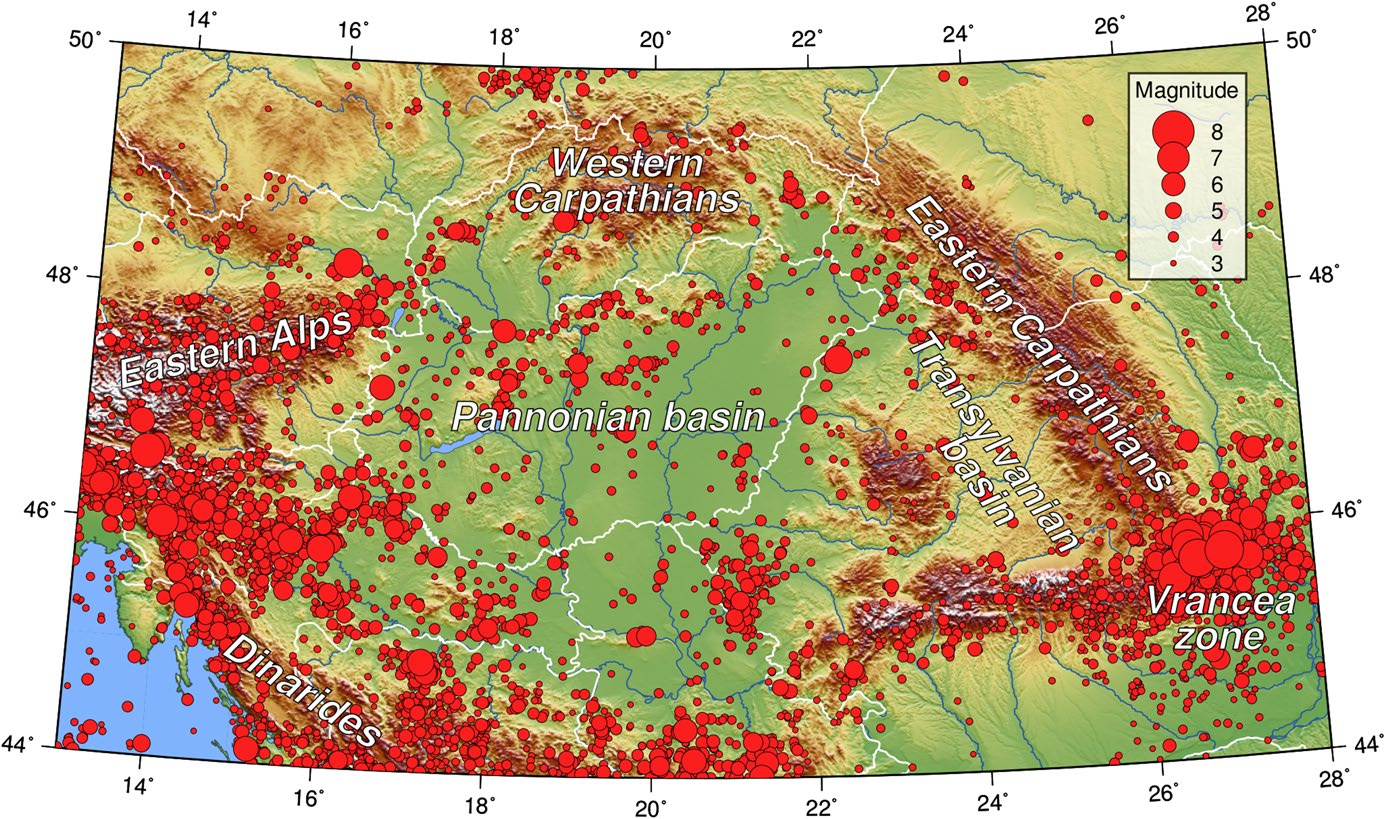
\includegraphics[width=\textwidth]{pannon_earthquakes.png}
        
        Figure from \cite{Matenco2018}.
    \end{minipage}
    \begin{minipage}[c]{0.45\textwidth}
        \pause
        \textbf{TropoTransylvania project:}
        \begin{itemize}
            \pause
            \item gedynamically active area: earthquakes, (post-)volcanism, salt tectonics (Praid)
            \pause
            \item natural geodynamic laboratory
            \pause
            \item investigate the Tansylvanian basin and the Vrancea zone
            \pause
            \item multidisciplinary: \pause seismology, \pause volcanology (post-volcanic, activity),
                  \pause mineralogy, \pause geology \pause geophysics \pause and geodesy.
        \end{itemize}
    \end{minipage}
\end{frame}

\begin{frame}{TopoTransylvania project - reflector networks}
    \begin{minipage}[c]{0.625\textwidth}
        \fig{praid_ciomadul.png}
    \end{minipage}
    \hspace{10pt}
    \begin{minipage}[c]{0.275\textwidth}
        %
    \end{minipage}
\end{frame}

\begin{frame}{TopoTransylvania project - reflector networks}
    \begin{minipage}[c]{0.625\textwidth}
        \fig{parajd_3D_mod.png}
    \end{minipage}
    \hspace{10pt}
    \begin{minipage}[c]{0.275\textwidth}
        \begin{itemize}
            \pause
            \item Largest salt diapir in Central Europe.
            \pause
            \item Salt mining $\rightarrow$ possible vertical movements.
            \pause
            \item Reflectors already installed.
        \end{itemize}
    \end{minipage}
\end{frame}

\begin{frame}{TopoTransylvania project - reflector networks}
    \begin{minipage}[c]{0.425\textwidth}
        \fig{csomad_network_alpha.png}
    \end{minipage}
    \hspace{10pt}
    \begin{minipage}[c]{0.475\textwidth}
        \begin{itemize}
            \pause
            \item Ciomadul volcano.
            \pause
            \item Dormant, possible reactivation? Magnetotelluric measurments
                  $\rightarrow$ magma chamber.
            \pause
            \item Reflectors to be installed in the following months.
        \end{itemize}
    \end{minipage}
\end{frame}

\begin{frame}{Summary}
    \begin{itemize}
        \pause
        \item InSAR is a very powerful technique for surface deformation detection,
        \pause
        \item compensation of InSAR drawbacks with artificial backscattering objects, reflectors,
        \pause
        \item monitoring of long-term, ``slow'',  geodynamic deformation processes.
    \end{itemize}
\end{frame}

\begin{frame}
    \centering
    {\Huge \color{red!65!black} \textbf{Thank you for your attetnion!}}
\end{frame}

\backupbegin

\section*{Backup}

\begin{frame}{Bibliography}
    \bibliographystyle{plain}
    \bibliography{/home/istvan/insar/insar}    
\end{frame}

\begin{frame}{Reflectors at Priad, Romania}
    \begin{figure}[H]
        \centering
        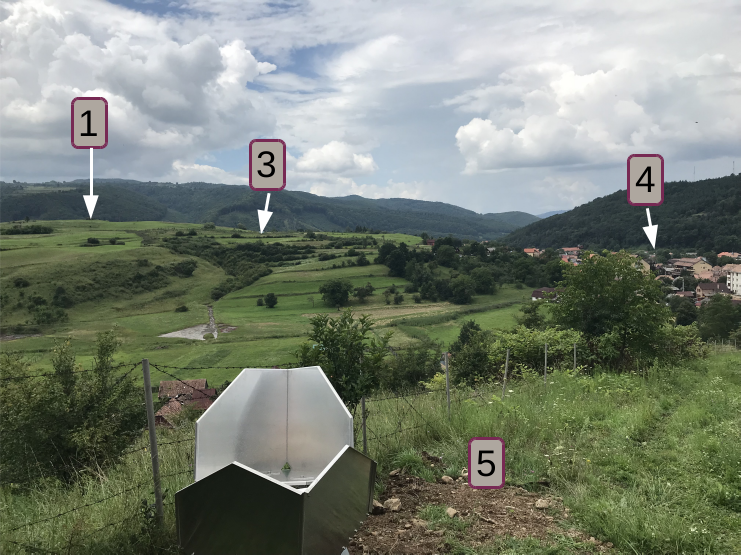
\includegraphics[width=0.625\textwidth]{praid_refl.png}
    \end{figure}
\end{frame}

\backupend

\end{document}
